
%% bare_conf.tex
%% V1.3
%% 2007/01/11
%% by Michael Shell
%% See:
%% http://www.michaelshell.org/
%% for current contact information.
%%
%% This is a skeleton file demonstrating the use of IEEEtran.cls
%% (requires IEEEtran.cls version 1.7 or later) with an IEEE conference paper.
%%
%% Support sites:
%% http://www.michaelshell.org/tex/ieeetran/
%% http://www.ctan.org/tex-archive/macros/latex/contrib/IEEEtran/
%% and
%% http://www.ieee.org/

%%*************************************************************************
%% Legal Notice:
%% This code is offered as-is without any warranty either expressed or
%% implied; without even the implied warranty of MERCHANTABILITY or
%% FITNESS FOR A PARTICULAR PURPOSE! 
%% User assumes all risk.
%% In no event shall IEEE or any contributor to this code be liable for
%% any damages or losses, including, but not limited to, incidental,
%% consequential, or any other damages, resulting from the use or misuse
%% of any information contained here.
%%
%% All comments are the opinions of their respective authors and are not
%% necessarily endorsed by the IEEE.
%%
%% This work is distributed under the LaTeX Project Public License (LPPL)
%% ( http://www.latex-project.org/ ) version 1.3, and may be freely used,
%% distributed and modified. A copy of the LPPL, version 1.3, is included
%% in the base LaTeX documentation of all distributions of LaTeX released
%% 2003/12/01 or later.
%% Retain all contribution notices and credits.
%% ** Modified files should be clearly indicated as such, including  **
%% ** renaming them and changing author support contact information. **
%%
%% File list of work: IEEEtran.cls, IEEEtran_HOWTO.pdf, bare_adv.tex,
%%                    bare_conf.tex, bare_jrnl.tex, bare_jrnl_compsoc.tex
%%*************************************************************************

% *** Authors should verify (and, if needed, correct) their LaTeX system  ***
% *** with the testflow diagnostic prior to trusting their LaTeX platform ***
% *** with production work. IEEE's font choices can trigger bugs that do  ***
% *** not appear when using other class files.                            ***
% The testflow support page is at:
% http://www.michaelshell.org/tex/testflow/



% Note that the a4paper option is mainly intended so that authors in
% countries using A4 can easily print to A4 and see how their papers will
% look in print - the typesetting of the document will not typically be
% affected with changes in paper size (but the bottom and side margins will).
% Use the testflow package mentioned above to verify correct handling of
% both paper sizes by the user's LaTeX system.
%
% Also note that the "draftcls" or "draftclsnofoot", not "draft", option
% should be used if it is desired that the figures are to be displayed in
% draft mode.
%
\documentclass[10pt, conference, compsocconf]{IEEEtran}
% Add the compsocconf option for Computer Society conferences.
%
% If IEEEtran.cls has not been installed into the LaTeX system files,
% manually specify the path to it like:
% \documentclass[conference]{../sty/IEEEtran}

% Packages
\usepackage[pdftex]{graphicx}

% for tables (use if required!)
\usepackage{setspace}
\usepackage{longtable}
\usepackage{colortbl}
\usepackage{array}
\usepackage{ragged2e}
\usepackage{lscape}
\usepackage{tabularx}
\usepackage{multirow}
\usepackage{booktabs}
\usepackage{url} 

%Anpassung der Namen f\"ur Abbildung und Tabelle
\usepackage[figurename={Abbildung},tablename={Tabelle}]{caption}

% Better handling of floats
\usepackage{float}

\newcolumntype{w}[1]{>{\raggedleft\hspace{0pt}}p{#1}}
\newcolumntype{x}[1]{>{\centering\hspace{0pt}}p{#1}}


% Set spaces between and after floats here:
\setlength{\textfloatsep}{8pt} % Vertical space below (above) [t] ([b]) floats


\newcommand{\conforms}{\mathrel{\widehat{=}}}


% correct bad hyphenation here
\hyphenation{}



% Some very useful LaTeX packages include:
% (uncomment the ones you want to load)


% *** MISC UTILITY PACKAGES ***
%
%\usepackage{ifpdf}
% Heiko Oberdiek's ifpdf.sty is very useful if you need conditional
% compilation based on whether the output is pdf or dvi.
% usage:
% \ifpdf
%   % pdf code
% \else
%   % dvi code
% \fi
% The latest version of ifpdf.sty can be obtained from:
% http://www.ctan.org/tex-archive/macros/latex/contrib/oberdiek/
% Also, note that IEEEtran.cls V1.7 and later provides a builtin
% \ifCLASSINFOpdf conditional that works the same way.
% When switching from latex to pdflatex and vice-versa, the compiler may
% have to be run twice to clear warning/error messages.






% *** CITATION PACKAGES ***
%
%\usepackage{cite}
% cite.sty was written by Donald Arseneau
% V1.6 and later of IEEEtran pre-defines the format of the cite.sty package
% \cite{} output to follow that of IEEE. Loading the cite package will
% result in citation numbers being automatically sorted and properly
% "compressed/ranged". e.g., [1], [9], [2], [7], [5], [6] without using
% cite.sty will become [1], [2], [5]--[7], [9] using cite.sty. cite.sty's
% \cite will automatically add leading space, if needed. Use cite.sty's
% noadjust option (cite.sty V3.8 and later) if you want to turn this off.
% cite.sty is already installed on most LaTeX systems. Be sure and use
% version 4.0 (2003-05-27) and later if using hyperref.sty. cite.sty does
% not currently provide for hyperlinked citations.
% The latest version can be obtained at:
% http://www.ctan.org/tex-archive/macros/latex/contrib/cite/
% The documentation is contained in the cite.sty file itself.






% *** GRAPHICS RELATED PACKAGES ***
%
\ifCLASSINFOpdf
  % \usepackage[pdftex]{graphicx}
  % declare the path(s) where your graphic files are
  % \graphicspath{{../pdf/}{../jpeg/}}
  % and their extensions so you won't have to specify these with
  % every instance of \includegraphics
  % \DeclareGraphicsExtensions{.pdf,.jpeg,.png}
\else
  % or other class option (dvipsone, dvipdf, if not using dvips). graphicx
  % will default to the driver specified in the system graphics.cfg if no
  % driver is specified.
  % \usepackage[dvips]{graphicx}
  % declare the path(s) where your graphic files are
  % \graphicspath{{../eps/}}
  % and their extensions so you won't have to specify these with
  % every instance of \includegraphics
  % \DeclareGraphicsExtensions{.eps}
\fi
% graphicx was written by David Carlisle and Sebastian Rahtz. It is
% required if you want graphics, photos, etc. graphicx.sty is already
% installed on most LaTeX systems. The latest version and documentation can
% be obtained at: 
% http://www.ctan.org/tex-archive/macros/latex/required/graphics/
% Another good source of documentation is "Using Imported Graphics in
% LaTeX2e" by Keith Reckdahl which can be found as epslatex.ps or
% epslatex.pdf at: http://www.ctan.org/tex-archive/info/
%
% latex, and pdflatex in dvi mode, support graphics in encapsulated
% postscript (.eps) format. pdflatex in pdf mode supports graphics
% in .pdf, .jpeg, .png and .mps (metapost) formats. Users should ensure
% that all non-photo figures use a vector format (.eps, .pdf, .mps) and
% not a bitmapped formats (.jpeg, .png). IEEE frowns on bitmapped formats
% which can result in "jaggedy"/blurry rendering of lines and letters as
% well as large increases in file sizes.
%
% You can find documentation about the pdfTeX application at:
% http://www.tug.org/applications/pdftex





% *** MATH PACKAGES ***
%
%\usepackage[cmex10]{amsmath}
% A popular package from the American Mathematical Society that provides
% many useful and powerful commands for dealing with mathematics. If using
% it, be sure to load this package with the cmex10 option to ensure that
% only type 1 fonts will utilized at all point sizes. Without this option,
% it is possible that some math symbols, particularly those within
% footnotes, will be rendered in bitmap form which will result in a
% document that can not be IEEE Xplore compliant!
%
% Also, note that the amsmath package sets \interdisplaylinepenalty to 10000
% thus preventing page breaks from occurring within multiline equations. Use:
%\interdisplaylinepenalty=2500
% after loading amsmath to restore such page breaks as IEEEtran.cls normally
% does. amsmath.sty is already installed on most LaTeX systems. The latest
% version and documentation can be obtained at:
% http://www.ctan.org/tex-archive/macros/latex/required/amslatex/math/





% *** SPECIALIZED LIST PACKAGES ***
%
%\usepackage{algorithmic}
% algorithmic.sty was written by Peter Williams and Rogerio Brito.
% This package provides an algorithmic environment fo describing algorithms.
% You can use the algorithmic environment in-text or within a figure
% environment to provide for a floating algorithm. Do NOT use the algorithm
% floating environment provided by algorithm.sty (by the same authors) or
% algorithm2e.sty (by Christophe Fiorio) as IEEE does not use dedicated
% algorithm float types and packages that provide these will not provide
% correct IEEE style captions. The latest version and documentation of
% algorithmic.sty can be obtained at:
% http://www.ctan.org/tex-archive/macros/latex/contrib/algorithms/
% There is also a support site at:
% http://algorithms.berlios.de/index.html
% Also of interest may be the (relatively newer and more customizable)
% algorithmicx.sty package by Szasz Janos:
% http://www.ctan.org/tex-archive/macros/latex/contrib/algorithmicx/




% *** ALIGNMENT PACKAGES ***
%
%\usepackage{array}
% Frank Mittelbach's and David Carlisle's array.sty patches and improves
% the standard LaTeX2e array and tabular environments to provide better
% appearance and additional user controls. As the default LaTeX2e table
% generation code is lacking to the point of almost being broken with
% respect to the quality of the end results, all users are strongly
% advised to use an enhanced (at the very least that provided by array.sty)
% set of table tools. array.sty is already installed on most systems. The
% latest version and documentation can be obtained at:
% http://www.ctan.org/tex-archive/macros/latex/required/tools/


%\usepackage{mdwmath}
%\usepackage{mdwtab}
% Also highly recommended is Mark Wooding's extremely powerful MDW tools,
% especially mdwmath.sty and mdwtab.sty which are used to format equations
% and tables, respectively. The MDWtools set is already installed on most
% LaTeX systems. The lastest version and documentation is available at:
% http://www.ctan.org/tex-archive/macros/latex/contrib/mdwtools/


% IEEEtran contains the IEEEeqnarray family of commands that can be used to
% generate multiline equations as well as matrices, tables, etc., of high
% quality.


%\usepackage{eqparbox}
% Also of notable interest is Scott Pakin's eqparbox package for creating
% (automatically sized) equal width boxes - aka "natural width parboxes".
% Available at:
% http://www.ctan.org/tex-archive/macros/latex/contrib/eqparbox/





% *** SUBFIGURE PACKAGES ***
%\usepackage[tight,footnotesize]{subfigure}
% subfigure.sty was written by Steven Douglas Cochran. This package makes it
% easy to put subfigures in your figures. e.g., "Figure 1a and 1b". For IEEE
% work, it is a good idea to load it with the tight package option to reduce
% the amount of white space around the subfigures. subfigure.sty is already
% installed on most LaTeX systems. The latest version and documentation can
% be obtained at:
% http://www.ctan.org/tex-archive/obsolete/macros/latex/contrib/subfigure/
% subfigure.sty has been superceeded by subfig.sty.



%\usepackage[caption=false]{caption}
%\usepackage[font=footnotesize]{subfig}
% subfig.sty, also written by Steven Douglas Cochran, is the modern
% replacement for subfigure.sty. However, subfig.sty requires and
% automatically loads Axel Sommerfeldt's caption.sty which will override
% IEEEtran.cls handling of captions and this will result in nonIEEE style
% figure/table captions. To prevent this problem, be sure and preload
% caption.sty with its "caption=false" package option. This is will preserve
% IEEEtran.cls handing of captions. Version 1.3 (2005/06/28) and later 
% (recommended due to many improvements over 1.2) of subfig.sty supports
% the caption=false option directly:
%\usepackage[caption=false,font=footnotesize]{subfig}
%
% The latest version and documentation can be obtained at:
% http://www.ctan.org/tex-archive/macros/latex/contrib/subfig/
% The latest version and documentation of caption.sty can be obtained at:
% http://www.ctan.org/tex-archive/macros/latex/contrib/caption/




% *** FLOAT PACKAGES ***
%
%\usepackage{fixltx2e}
% fixltx2e, the successor to the earlier fix2col.sty, was written by
% Frank Mittelbach and David Carlisle. This package corrects a few problems
% in the LaTeX2e kernel, the most notable of which is that in current
% LaTeX2e releases, the ordering of single and double column floats is not
% guaranteed to be preserved. Thus, an unpatched LaTeX2e can allow a
% single column figure to be placed prior to an earlier double column
% figure. The latest version and documentation can be found at:
% http://www.ctan.org/tex-archive/macros/latex/base/



%\usepackage{stfloats}
% stfloats.sty was written by Sigitas Tolusis. This package gives LaTeX2e
% the ability to do double column floats at the bottom of the page as well
% as the top. (e.g., "\begin{figure*}[!b]" is not normally possible in
% LaTeX2e). It also provides a command:
%\fnbelowfloat
% to enable the placement of footnotes below bottom floats (the standard
% LaTeX2e kernel puts them above bottom floats). This is an invasive package
% which rewrites many portions of the LaTeX2e float routines. It may not work
% with other packages that modify the LaTeX2e float routines. The latest
% version and documentation can be obtained at:
% http://www.ctan.org/tex-archive/macros/latex/contrib/sttools/
% Documentation is contained in the stfloats.sty comments as well as in the
% presfull.pdf file. Do not use the stfloats baselinefloat ability as IEEE
% does not allow \baselineskip to stretch. Authors submitting work to the
% IEEE should note that IEEE rarely uses double column equations and
% that authors should try to avoid such use. Do not be tempted to use the
% cuted.sty or midfloat.sty packages (also by Sigitas Tolusis) as IEEE does
% not format its papers in such ways.





% *** PDF, URL AND HYPERLINK PACKAGES ***
%
%\usepackage{url}
% url.sty was written by Donald Arseneau. It provides better support for
% handling and breaking URLs. url.sty is already installed on most LaTeX
% systems. The latest version can be obtained at:
% http://www.ctan.org/tex-archive/macros/latex/contrib/misc/
% Read the url.sty source comments for usage information. Basically,
% \url{my_url_here}.





% *** Do not adjust lengths that control margins, column widths, etc. ***
% *** Do not use packages that alter fonts (such as pslatex).         ***
% There should be no need to do such things with IEEEtran.cls V1.6 and later.
% (Unless specifically asked to do so by the journal or conference you plan
% to submit to, of course. )


% correct bad hyphenation here
\hyphenation{op-tical net-works semi-conduc-tor}


\begin{document}
%
% paper title
% can use linebreaks \\ within to get better formatting as desired
\title{Entwicklung einer Einkaufslisten-App}


% author names and affiliations
% use a multiple column layout for up to two different
% affiliations

\author{\IEEEauthorblockN{Markus H\"ul\ss}
\IEEEauthorblockA{
Email: huma1200@stud.hs-coburg.de}
\\
\IEEEauthorblockN{Tanja M\"ogn}
\IEEEauthorblockA{
Email: mota1200@stud.hs-coburg.de}
\and
\IEEEauthorblockN{Malcolm K\"ogler}
\IEEEauthorblockA{
Email: koma1200@stud.hs-coburg.de}
\\
\IEEEauthorblockN{Daniel M\"uller}
\IEEEauthorblockA{
Email: muda1200@stud.hs-coburg.de}
}

% conference papers do not typically use \thanks and this command
% is locked out in conference mode. If really needed, such as for
% the acknowledgment of grants, issue a \IEEEoverridecommandlockouts
% after \documentclass

% for over three affiliations, or if they all won't fit within the width
% of the page, use this alternative format:
% 
%\author{\IEEEauthorblockN{Michael Shell\IEEEauthorrefmark{1},
%Homer Simpson\IEEEauthorrefmark{2},
%James Kirk\IEEEauthorrefmark{3}, 
%Montgomery Scott\IEEEauthorrefmark{3} and
%Eldon Tyrell\IEEEauthorrefmark{4}}
%\IEEEauthorblockA{\IEEEauthorrefmark{1}School of Electrical and Computer Engineering\\
%Georgia Institute of Technology,
%Atlanta, Georgia 30332--0250\\ Email: see http://www.michaelshell.org/contact.html}
%\IEEEauthorblockA{\IEEEauthorrefmark{2}Twentieth Century Fox, Springfield, USA\\
%Email: homer@thesimpsons.com}
%\IEEEauthorblockA{\IEEEauthorrefmark{3}Starfleet Academy, San Francisco, California 96678-2391\\
%Telephone: (800) 555--1212, Fax: (888) 555--1212}
%\IEEEauthorblockA{\IEEEauthorrefmark{4}Tyrell Inc., 123 Replicant Street, Los Angeles, California 90210--4321}}




% use for special paper notices
%\IEEEspecialpapernotice{(Invited Paper)}




% make the title area
\maketitle


\begin{abstract}
Mangels Verf\"ugbarkeit von multitplattformf\"ahigen Apps zur Verwaltung von Einkaufslisten, entstand die Idee eine solche App zu entwicklen. Um den Entwicklungsaufwand m\"oglichst gering zu halten und nicht f\"ur jede Plattform separat eine App zu programmieren, entschieden wir uns f\"ur das Framework Phonegap. Dieses Paper besch\"aftigt sich mit der Konzeption und Entwicklung der App.   
\end{abstract}

%\begin{IEEEkeywords}
%
%\end{IEEEkeywords}


% For peer review papers, you can put extra information on the cover
% page as needed:
% \ifCLASSOPTIONpeerreview
% \begin{center} \bfseries EDICS Category: 3-BBND \end{center}
% \fi
%
% For peerreview papers, this IEEEtran command inserts a page break and
% creates the second title. It will be ignored for other modes.
\IEEEpeerreviewmaketitle



\section{Einleitung}
% no \IEEEPARstart
Immer pr\"asent und nicht mehr aus dem Alltag wegzudenken, unterst\"utzt  uns das Smartphone heute schon bei der Organisation und Kommunikation. Vor einigen Jahren hat man vor dem Einkauf noch schnell einen Einkaufszettel geschrieben. Aber wie schnell war der Zettel doch in der Tasche spurlos verschwunden, obwohl man sich so sicher war, den Zettel eingepackt zu haben. Heutzutage bietet sich das Smartphone als M\"oglichkeit an, einen Einkaufszettel zu speichern. Das bietet unter anderem die M\"oglichkeit den Einkaufszettel zu jeder Zeit zu erweitern, oder ihn mit anderen zu teilen. 
Ziel dieser Arbeit ist es eine App zur Verwaltung von Einkaufszetteln zu entwickeln.
Diese soll es erm\"oglichen erstellte Einkaufszettel mit anderen zu teilen.
Die jeweilige Plattform des App-Benutzers sollte dabei kein Hindernis darstellen.
Die Projektgruppe wurde in zwei Teams aufgeteilt. 
Ein Team war f\"ur die Frontend-Entwicklung zust\"andig, das andere f\"ur das Backend. 
Der Programmcode wurde mittels des Versionierungssystems GIT verwaltet. 
Grafiken wurden mit Balsamiq und MS Visio 2013 erstellt. 
Die Kommunikation erfolgte teils pers\"onlich, teils \"uber E-Mails.

Am Anfang wurde eine Konkurrenzanalyse angefertigt um einen \"Uberblick \"uber die bereits am Markt verf\"ugbaren Apps zu erm\"oglichen.
Als n\"achstes wird die Erstellung von Prototypen anhand von Mockups beschrieben, welche die Grundlage f\"ur die Entwicklung bildeten.
Darauffolgend werden die verwendeten Technologien in Frontend und Backend im Zusammehang mit dem Nutzen in der App vorgestellt. Zuletzt werden in einer Zusammenfassung die Projekterfolge und Misserfolge aufgezeigt.

\section{Konkurrenzanalyse}
Um sich einen \"Uberblick \"uber vorhandene Apps zu verschaffen, wurde eine Konkurrenzanalyse erstellt.
Diese Konkurrenzanalyse beschr\"ankt sich auf native Apps und l\"asst Cloud-basierte L\"osungen au{\ss}en vor.
Zu diesem Zweck wurden die Top-Apps aus den App-Stores f\"ur die Plattformen Android, IOS und Windows Phone miteinander verglichen.
Um die Apps miteinander vergleichen zu k\"onnen, wurden drei Merkmale definiert. 
Diese Merkmale waren Plattformunabh\"angigkeit bzw. Multiplattformf\"ahigkeit, 
die M\"oglichkeit Einkaufslisten mit anderen Leuten zu Teilen sowie eine zentrale Datenhaltung mit Sychronisierung der Daten \"uber mehrere Ger\"ate hinweg.

Am Markt gibt es mittelerweile mehrere Apps die darauf spezialisiert sind Einkaufslisten zu verwalten.
Nur eine App bietet eine native Implementierung f\"ur die oben genannten Plattformen. Einige Apps bieten eine reduzierte Multiplattformf\"ahigkeit in dem Sinne, dass ein Webservice zu Verf\"ugung gestellt wird \"uber dem auf die Daten zugegriffen werden kann.
Die meisten Apps bieten ein Backbone zur zentralen Datenhaltung.
Nur wenige Apps bieten die M\"oglichkeit Einkaufslisten mit anderen zu teilen. Diese F\"ahigkeit ist teilweise darauf beschr\"ankt eine Einkaufsliste per E-Mail zu 
verschicken.

Einzig allein eine App deckt alle drei definierten Merkmale ab. 
F\"ur die Plattform Windows Phone ist keine App mit den definierten Merkmalen vorhanden.
Bei Android und IOS ist die Situation etwas besser, allerdings ist auch hier Potenzial vorhanden.

\section{Mockups}
Zu Beginn der Entwicklung wurde eine M\"oglichkeit gesucht schnell einen Prototypen der App zu entwickeln.
Zu diesem Zweck wurden Mockups f\"ur das Frontend erstellt. 
Diese wurden in Teamarbeit entworfen und somit hatte jeder im Team eine Vorstellung wie die App sp\"ater aussehen soll.
\begin{figure}[h!]
	\centering
	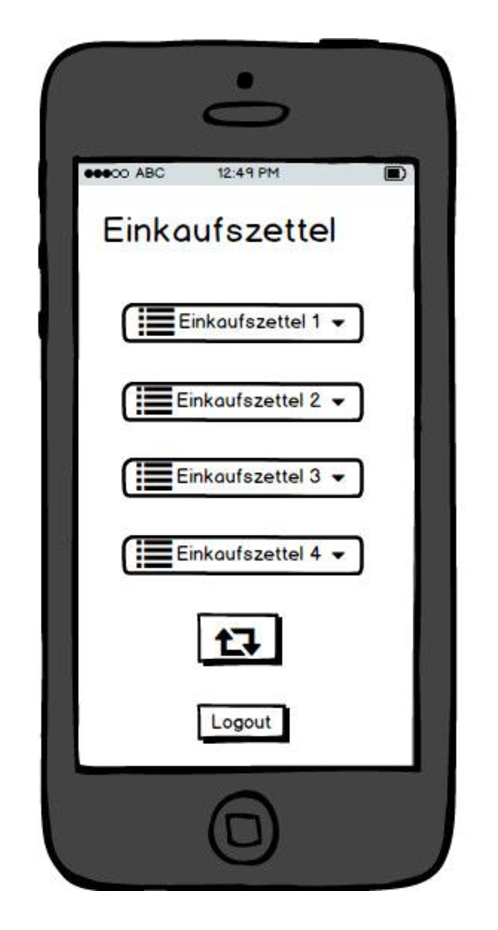
\includegraphics[scale=0.3]{./Bilder_Zeichnungen/Uebersicht.pdf}
	\caption{Einzelansicht}
	\label{fig:Mockup_Einzelansicht}
\end{figure}
In Abbildung~\ref{fig:Mockup_Einzelansicht} ist ein Beispiel f\"ur ein solches Mockup zu sehen. Die Abbildung~\ref{fig:Mockup_Einzelansicht} zeigt die Ansicht eines Einkaufszettels mit den zugeh\"origen Steuerelementen.

\section{Frontend}
Ein wichtiges Ziel ist es eine plattform- und aufl\"osungsunabh\"angige Darstellung zu erm\"oglichen. 
Dabei soll das Frontend nicht f\"ur jede Plattform separat entwickelt werden.
Dies soll sowohl den Zeitaufwand, als auch potentielle Fehlerquellen zu verringern. 
Der Browser dient als Grundlage für die Darstellung. 
Somit ist eine einfache Darstellung auf mobilen Ger\"aten und Desktop PC's m\"oglich.
Dieser Abschnitt befasst sich mit den beiden Komponenten "Phonegap" und "jQuery mobile".

\subsection{Phonegap}
Die auf dem Markt vorhandenen Applikationen entwickeln f\"ur Android, iPhone und Windows Phone jeweils separate native Apps. 
Das erfordert tiefgehendes KnowHow f\"ur die einzelnen Plattformen und weitergehende separate Behandlung von Fehler- und Change-Requests. 
Aus diesem Grund wird bei der Entwicklung der App auf Phonegap gesetzt. Phonegap ist ein Framework zum Erstellen von nativen Anwendungen f\"ur die g\"angigsten mobilen Plattformen durch die Verwendung von HTML5.
Das Konzept von Phonegap ist auf einer Seite das Frontend einer Anwendung \"uber eine angezeigte Webseite im Browser zu realiseren. 
Auf der anderen Seite stellt es zus\"atzlich Javasript API's bereit die einem Zugriff auf bestimmte Hardware wie der Kamera oder bestimmte Sensoren erm\"oglichen. 
Auch kann auf Events wie beispielsweise eine schwache Funkverbindung reagiert werden. 
Somit sind Funktionalit\"aten nativer Apps gegeben, ohne sich intensiv mit der Architektur jeglicher Zielplattformen auseinanderzusetzen.
Zus\"atzlich baut Phonegap am Ende aus diesen Komponenten eine native App, welche sich in dem dementsprechenden Store anbieten l\"asst.

\subsection{jQuery Mobile}
Ein zus\"atzliches Problem neben den unterschiedlichen Plattformen, ist die Vielzahl an unterschiedlichen Browsern und Displayaufl\"osungen der Endger\"ate. 
Die Anwendung soll ein einheitliches Design, unabh\"angig von Browser und Aufl\"osung besitzen. 
Ein Benutzer soll sich nicht bei einem Wechseln zwischen einem normalen und einem mobilen Browser bei der Bedienung umgew\"ohnen m\"u{\ss}en. 
Um dieser Anforderung nachzukommen wird auf das jQuery Mobile Framework zur\"uckgegriffen.
Es erm\"oglicht eine einfache Umsetzung von Webseiten mit einem responsive Design und bietet eine gro{\ss}e Auswahl unterst\"utzter Browser (sowohl mobile, als auch non-mobile). 
Somit wird mit einer einzigen Version des Frontends eine gro{\ss}e Menge an Endger\"aten unterst\"utzt und tr\"agt zu einer schnellen Entwicklung der Anwendung bei. 
Zus\"atzlich ist es mit dem Multi-Page-Layout Konzept m\"oglich mit einer einzigen HTML-Seite alle Ansichten einer App darzustellen. Dadurch muss nicht bei jedem Wechsel einer Ansicht eine neue Seite heruntergeladen werden, womit sich die Performance verbessert und Traffic gespart wird. (Bisherige Quelle bisher nur die jQuery Mobile Website)

\section{Backend}
Ein weiteres wichtiges Ziel ist es eine endger\"ateunabh\"angige Datenspeicherung zu gew\"ahrleisten. 
Daf\"ur ist ein Backend das von \"uberall \"uber das Internet zu erreichen ist von n\"oten. 
F\"ur die Umsetzung des Projekts entschieden wir uns f\"ur einen einfachen Webserver und die Nutzung von PHP und MySQL zur Datenhaltung und f\"ur JSON nach dem ReST-Standart zur Kommunikation zwischen Anwendung und Backend.  
Dieser Abschnitt befasst sich mit den Komponenten PHP, MySQL und JSON, welche die Umsetzung der Anforderungen erm\"oglichen.

\subsection{PHP}
PHP wird im Backend verwendet um die Schnittstelle zwischen Anwendung und Datenbank auf dem Webserver zu stellen. PHP unterst\"utzt unz\"ahlige Datenbanktypen und ein breites Spektrum an Funktionalit\"aten zur Konvertierung in das JSON Format.

\subsection{MySQL}
MySQL ist ein weit verbreitetes relationales Datenbanksystem und kam vor allem wegen seiner plattformunabh\"angigkeit und der kostenfreien Nutzung unter der OpenSource-Lizenz zur Umsetzung der Datenbank in Frage. 
Bei der Auswahl spielte auch die M\"oglichkeit der Verwendung von verschiedenen Speicherssubsystemen eine Rolle. 
Durch die Verwendung von InnoDB stehen Rollback und Transaktionssicherungsm\"oglichkeiten zur Verf\"ugung, dies ist ein wichtiger Gesichtspunkt im Bezug auf Datensicherheit.

\begin{figure*}[t]
	\centering
	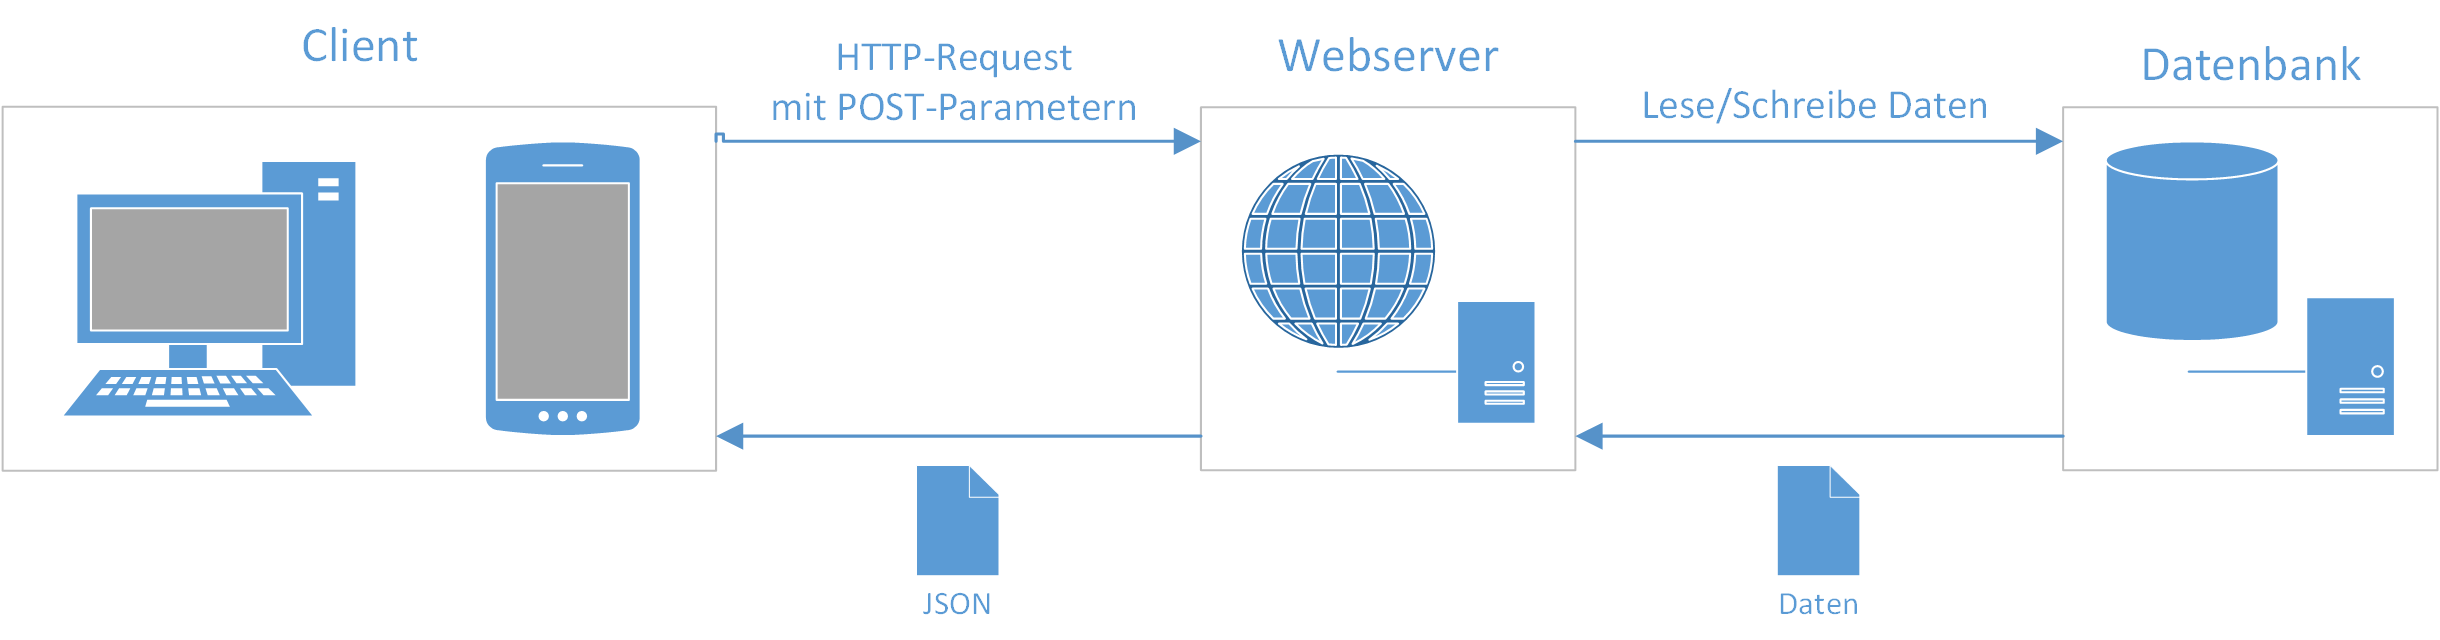
\includegraphics[width=0.9\textwidth]{./Bilder_Zeichnungen/Architektur.png}
	\caption{3-Wege-Architektur f\"ur die App}
	\label{fig:Architektur}
\end{figure*}

\subsection{JSON}
Aufgrund der Verwendung des auf Javascript basierenden Frameworks JQuery-Mobile zur Erstellung einer Webapp, lag die Verwendung von JSON als Format zum Datenaustausch zwischen Anwendung und Backend nahe. 
Dadurch ist es m\"oglich die Daten vom Backend ohne vorherige Konvertierung in der Anwendung. 
Mithilfe von PHP l\"asst sich so die Schnittstelle nach dem REST Programmierparadigma gestalten, die die geforderten Daten im JSON zur\"uckliefert. 

\section{Architektur}
{Damit die einzelnen Komponenten ordnungsgem\"a{\ss} so zusammenarbeiten, ben\"otigt es noch eine passende Architektur. Aufgrund der verwendeten Technologien wird eine Drei-Schichten-Architektur verwendet. Somit l\"asst sich eine Trennung von Pr\"asentation und Anwendungslogik realisieren.
	
Die Abbildung~\ref{fig:Architektur} zeigt den genauen Aufbau der Architektur. Ein Client sendet seine Aktion per HTTP-Request an den Webserver. Dieser holt geforderte Daten aus der Datenbank, oder \"andert diese. Die von der Datenbank erhaltenen Daten werden in das JSON Format konvertiert. Danach werden sie als Inhalt des HTTP-Response an den Client gesendet. Der genauere Ablauf ist im Abbildung~\ref{fig:Sequenzdiagramm} ersichtlich.

\begin{figure}[h!]
	\centering
	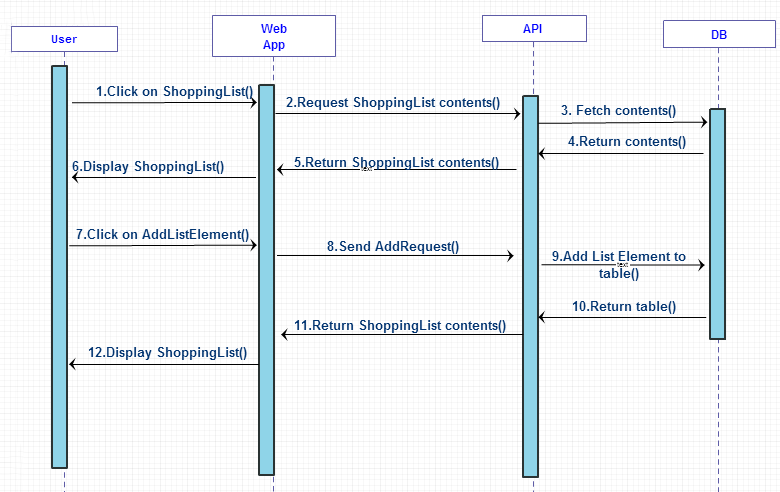
\includegraphics[width=0.45\textwidth]{./Bilder_Zeichnungen/Sequenzdiagramm.png}
	\caption{Sequenzdiagramm}
	\label{fig:Sequenzdiagramm}
\end{figure}

\section{Zusammenfassung}
Anmerkung Tanja: Hier ist vielleicht wichtig das wir reinschreiben, dass zwar Cordova und JQuery mobile ganz h\"ubsch sind, es aber trotzdem noch nicht das wahre vom Ei ist. Au{\ss}erdem sollten wir erw\"ahnen wo es Probleme gab.

\section {Ausblick (Anmerkung: Vielleicht noch erw\"ahnen inwiefern die Offline Benutzung realisiert werden kann, da das Grundkonzept eine persistente Datenspeicherung in einer zentralen Datenbank vorsieht.)}
Die App “HIER NAME EINF\"UGEN” besitzt bereits alle notwendigen Funktionen um eine Einkaufsliste zu erstellen, editieren und teilen. In der weiteren Entwicklung werden die Vorteile von Phonegap eingebaut. So wird beispielsweise ein Offline-Modus entwickelt, der es erm\"oglichen soll, die App auch ohne permanenten Internetverbindung zu nutzten. Das ist mit Phonegap m\"oglich, da man mit diesem Framework die Qualit\"at der Internetverbindung abfragen kann. Des weiteren ist eine intelligentere Unterst\"utzung der App in den Alltag gedacht. Die App soll beispielsweise den User benachrichtigen, falls eine ein anderer User in einer gemeinsamen Einkaufsliste einen Eintrag ge\"andert oder hinzugef\"ugt hat. Hier ist wichtig das unbedingt der native Benachrichtigungsmodus des Systems verwendet wird um so viel Usability wie m\"oglich zu gew\"ahrleisten. Ein weitere Verbesserung w\"are auch die permanenten Lokalisierung des Users und eine Reaktion der Einkaufslisten-App, wenn sich der User in der N\"ahe oder in einem Einkaufsladen befindet. Hiermit hebt sich die HIER NAME EINF\"UGEN von seinem Konkurrenten auf dem Markt ab.

%\section{Type style and Fonts}
%Wherever Times is specified, Times Roman or Times New Roman may be used. If neither is available on your system, please use the font closest in appearance to Times. Avoid using bit-mapped fonts if possible. True-Type 1 or Open Type fonts are preferred. Please embed symbol fonts, as well, for math, etc.


% An example of a floating figure using the graphicx package.
% Note that \label must occur AFTER (or within) \caption.
% For figures, \caption should occur after the \includegraphics.
% Note that IEEEtran v1.7 and later has special internal code that
% is designed to preserve the operation of \label within \caption
% even when the captionsoff option is in effect. However, because
% of issues like this, it may be the safest practice to put all your
% \label just after \caption rather than within \caption{}.
%
% Reminder: the "draftcls" or "draftclsnofoot", not "draft", class
% option should be used if it is desired that the figures are to be
% displayed while in draft mode.
%
%\begin{figure}[!t]
%\centering
%\includegraphics[width=2.5in]{myfigure}
% where an .eps filename suffix will be assumed under latex, 
% and a .pdf suffix will be assumed for pdflatex; or what has been declared
% via \DeclareGraphicsExtensions.
%\caption{Simulation Results}
%\label{fig_sim}
%\end{figure}

% Note that IEEE typically puts floats only at the top, even when this
% results in a large percentage of a column being occupied by floats.


% An example of a double column floating figure using two subfigures.
% (The subfig.sty package must be loaded for this to work.)
% The subfigure \label commands are set within each subfloat command, the
% \label for the overall figure must come after \caption.
% \hfil must be used as a separator to get equal spacing.
% The subfigure.sty package works much the same way, except \subfigure is
% used instead of \subfloat.
%
%\begin{figure*}[!t]
%\centerline{\subfloat[Case I]\includegraphics[width=2.5in]{subfigcase1}%
%\label{fig_first_case}}
%\hfil
%\subfloat[Case II]{\includegraphics[width=2.5in]{subfigcase2}%
%\label{fig_second_case}}}
%\caption{Simulation results}
%\label{fig_sim}
%\end{figure*}
%
% Note that often IEEE papers with subfigures do not employ subfigure
% captions (using the optional argument to \subfloat), but instead will
% reference/describe all of them (a), (b), etc., within the main caption.


% An example of a floating table. Note that, for IEEE style tables, the 
% \caption command should come BEFORE the table. Table text will default to
% \footnotesize as IEEE normally uses this smaller font for tables.
% The \label must come after \caption as always.
%
%\begin{table}[!t]
%% increase table row spacing, adjust to taste
%\renewcommand{\arraystretch}{1.3}
% if using array.sty, it might be a good idea to tweak the value of
% \extrarowheight as needed to properly center the text within the cells
%\caption{An Example of a Table}
%\label{table_example}
%\centering
%% Some packages, such as MDW tools, offer better commands for making tables
%% than the plain LaTeX2e tabular which is used here.
%\begin{tabular}{|c||c|}
%\hline
%One & Two\\
%\hline
%Three & Four\\
%\hline
%\end{tabular}
%\end{table}


% Note that IEEE does not put floats in the very first column - or typically
% anywhere on the first page for that matter. Also, in-text middle ("here")
% positioning is not used. Most IEEE journals/conferences use top floats
% exclusively. Note that, LaTeX2e, unlike IEEE journals/conferences, places
% footnotes above bottom floats. This can be corrected via the \fnbelowfloat
% command of the stfloats package.




% conference papers do not normally have an appendix


% use section* for acknowledgement
%\section*{Acknowledgment}
%
%
%The authors would like to thank...
%more thanks here


% trigger a \newpage just before the given reference
% number - used to balance the columns on the last page
% adjust value as needed - may need to be readjusted if
% the document is modified later
%\IEEEtriggeratref{8}
% The "triggered" command can be changed if desired:
%\IEEEtriggercmd{\enlargethispage{-5in}}

% references section

% can use a bibliography generated by BibTeX as a .bbl file
% BibTeX documentation can be easily obtained at:
% http://www.ctan.org/tex-archive/biblio/bibtex/contrib/doc/
% The IEEEtran BibTeX style support page is at:
% http://www.michaelshell.org/tex/ieeetran/bibtex/
%\bibliographystyle{IEEEtran}
% argument is your BibTeX string definitions and bibliography database(s)
%\bibliography{IEEEabrv,../bib/paper}
%
% <OR> manually copy in the resultant .bbl file
% set second argument of \begin to the number of references
% (used to reserve space for the reference number labels box)
%\begin{thebibliography}{1}

%\bibitem{IEEEhowto:kopka}
%H.~Kopka and P.~W. Daly, \emph{A Guide to \LaTeX}, 3rd~ed.\hskip 1em plus
%  0.5em minus 0.4em\relax Harlow, England: Addison-Wesley, 1999.

%\end{thebibliography}




% that's all folks
\end{document}


